Para analizar la efectividad y ecuanimidad de esta nueva forma de calcular el ranking vamos a realizar una serie de test a fin de obtener un analisis cuantitativo y cualitativo que nos permita compararlo con el clásico método de \textbf{WP}. \\
Con los test esperamos encontrar ventajas y desventajas de esta forma de medición, particularmente en escenarios donde no todos los participantes juegen la misma cantidad de partidos.
\\

Además realizaremos una comparación de los métodos de \textbf{Eliminación Gaussiana} y \textbf{Cholesky} para ver cual de los dos computa los rankings de manera mas eficiente.
\\

En esta sección solo presentaremos los experimentos realizados y los resultados obtenidos. Las conclusiones de cada experimento
las presentaremos en la seguiente sección. 


\subsection{Ranking}

Vamos a comparar la tabla de ranking obtenida a partir de un set de datos de la \textbf{ATP 2007}. Es decir calculamos el ranking a partir de la técnica \textbf{WP}, considerando partidos ganado / partidos jugados, a pesar de que no todos los jugadores hayan participado de la misma cantidad de partidos. Comparandolo con el \textbf{CMM} implementado con \textbf{Eliminación Gaussiana} y \textbf{Cholesky}. \\


\begin{figure}[H]
\centering
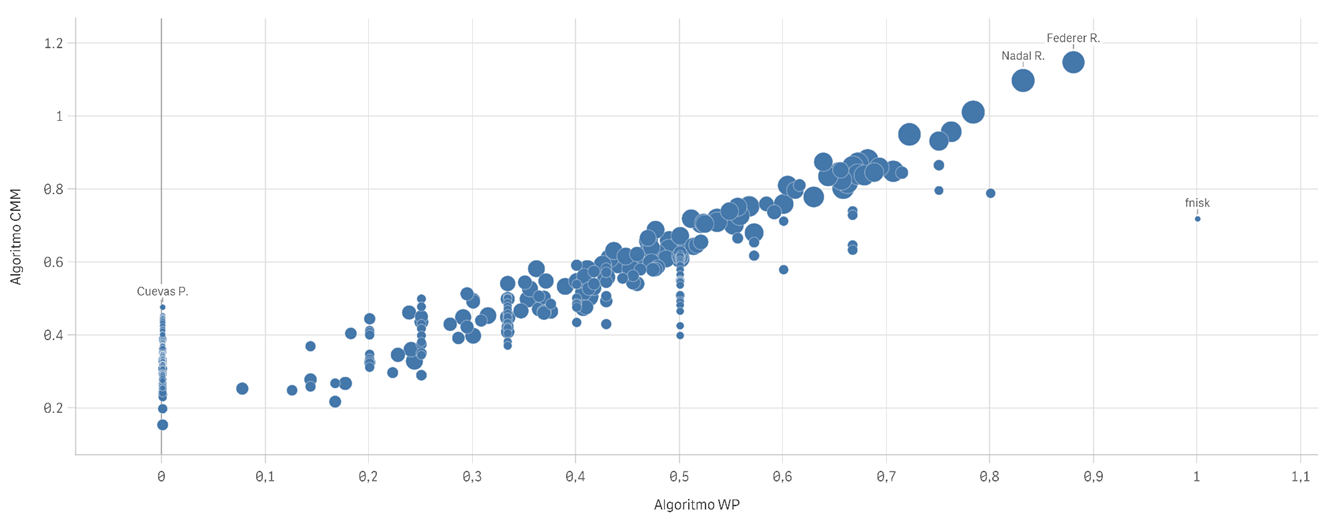
\includegraphics[width=1\textwidth]{IMG/Comparativa WP- CMM todos.png}
\caption{Rankings Calculados con las 3 tecnicas}
\label{fig:Comparacion de tecnicas}
\end{figure}

\\

Hemos realizado un zoom dentro del grafico para corroborar el nombre y posicion de ambos rankings.
\\

\begin{figure}[H]
\centering
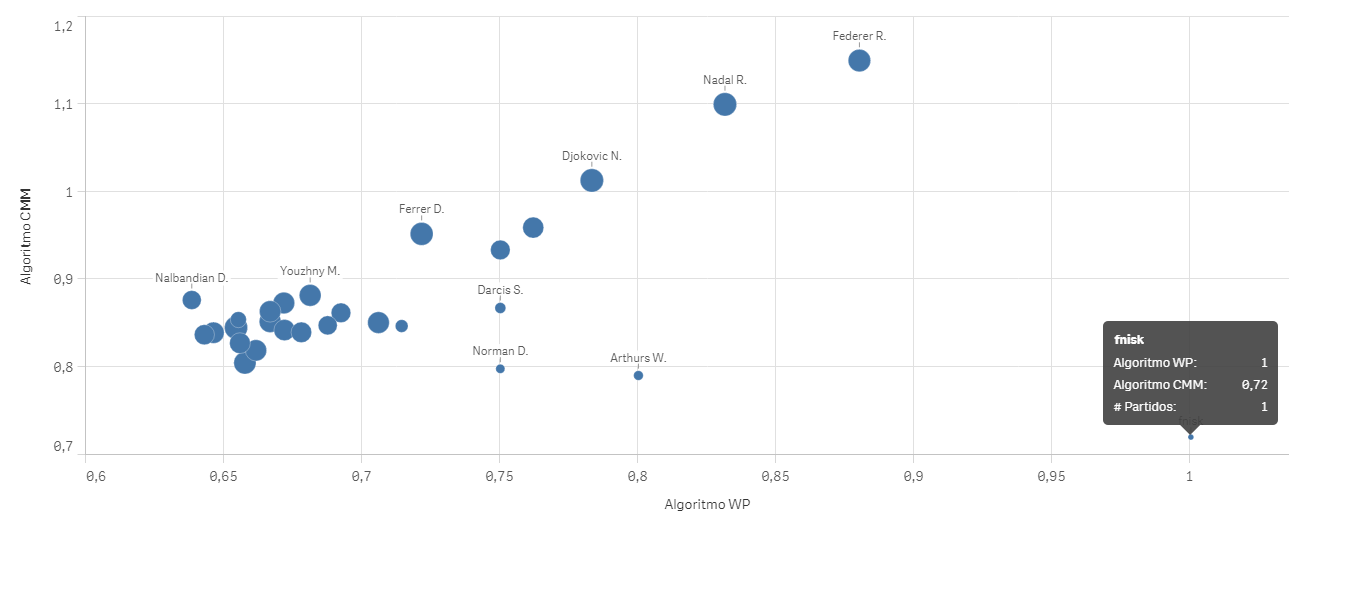
\includegraphics[width=1\textwidth]{IMG/comparativa WP - CMM zoom.png}
\caption{Zoom de las primeras posiciones}
\label{fig:Zoom de las primeras posiciones}
\end{figure}

\\

\subsection{¿Importa a quien se le gana?}


En el escenario que se utilize \textbf{WP} realmente no importa a que equipo se le gane, ya que todos los partidos tienen la misma importancia y se les asigna el mismo puntaje. Pero en el caso de \textbf{CMM} resulta mas interesante plantearse esta pregunta. \\

La hipótesis que tenemos es que tomando un equipo de mitad de tabla, que denominamos \textbf{medio} el hecho de que le gane al lider de la tabla va a mejorar mucho mas el ranking que derrotando al que ocupe la última posición. \\

Realizamos un test tomando al equipo \textbf{medio}, y agregando un partido victorioso contra el puntero y analizamos como se modifica su ranking. Luego tomamos la tabla inicial, es decir sin ganarle al puntero, y repetimos el experimento esta vez derrotando al último. \\

Presentamos los resultados obtenidos.

\\


******Aca van los graficos de: tabla inicial, perder contra el primero y perder contra el ultimo (sacando el partido con el primero)

\\




\subsection{¿Importa contra quien se pierde?}

Para verificar si importa contra que equipo se juega, proponemos el test de tomar un equipo que se encuentra por la mitad de la tabla. Por notación denominamos a este equipo como \textbf{medio}. \\

Para lograrlo calculamos un ranking a partir de un set de datos. Y luego generamos una nueva instancia enfrentando a \textbf{medio}contra el actual puntero y calculamos el nuevo ranking. Volvemos a tomar la primer instancia y lo enfrentamos contra el último, calculamos nuevamente el ranking y luego comparamos los tres rankings obtenidos. La premisa que tenemos del experimento es que el ranking del equipo \textbf{medio} no debería ser afectado por el rival contra el que perdió.\\

Este experimento lo calculamos usando la técnica de \textbf{CMM}, ya que considerar \textbf{WP} no afecta el resultado.

\\
A continuación presentamos los graficos obtenidos.

\\


******Aca van los graficos de: tabla inicial, perder contra el primero y perder contra el ultimo (sacando el partido con el primero)

\\



\subsection{Racha ganadora}

Para estudiar la ecuanimidad del \textbf{CMM} realizamos un experimento tomando al participante del \textbf{ATP 2007} que se encontraba en el último puesto y le asignamos una racha ganadora contra los primeros diez jugadores del ranking. \\

Además este test nos permite observar como la racha de un jugador afecta al ranking global y si ganandole a los mejores realmente escala una considerable cantidad de posiciones en el ranking. \\

A continuacion presentamos el ranking calculado construido de la siguiente manera: \\


\begin{itemize}
	\item Eje X el valor obtenido al ejecutar CMM implementado con Cholesky.
	\item Eje Y el valor obtenido al ejecutar CMM implementado con Eliminación Gaussiana.
	\item El tamaño de la burbuja es la cantidad de partidos jugados.
\end{itemize}

\\

\begin{figure}[H]
\centering
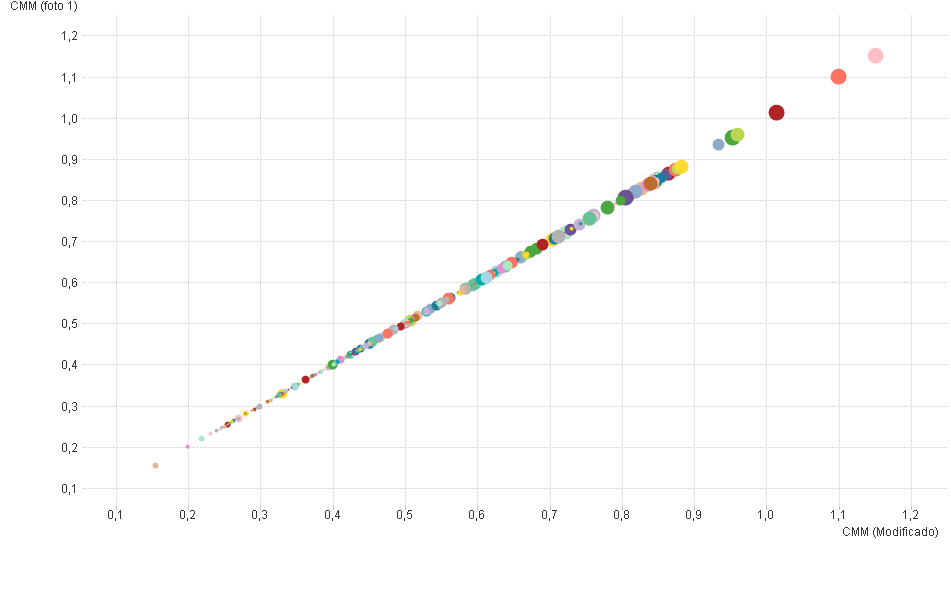
\includegraphics[width=1\textwidth]{IMG/comparativa cmm -cmm foto 0.png}
\caption{Zoom de las primeras posiciones}
\label{fig:Zoom de las primeras posiciones}
\end{figure}

\\
Y a continuación el ranking después de los 10 partidos: \\
\\
En el gráfico se observa mediante una flecha cual es la ganancia en Ranking que tiene el ultimo jugador al ganarle a los top 10.\\

\begin{figure}[H]
\centering
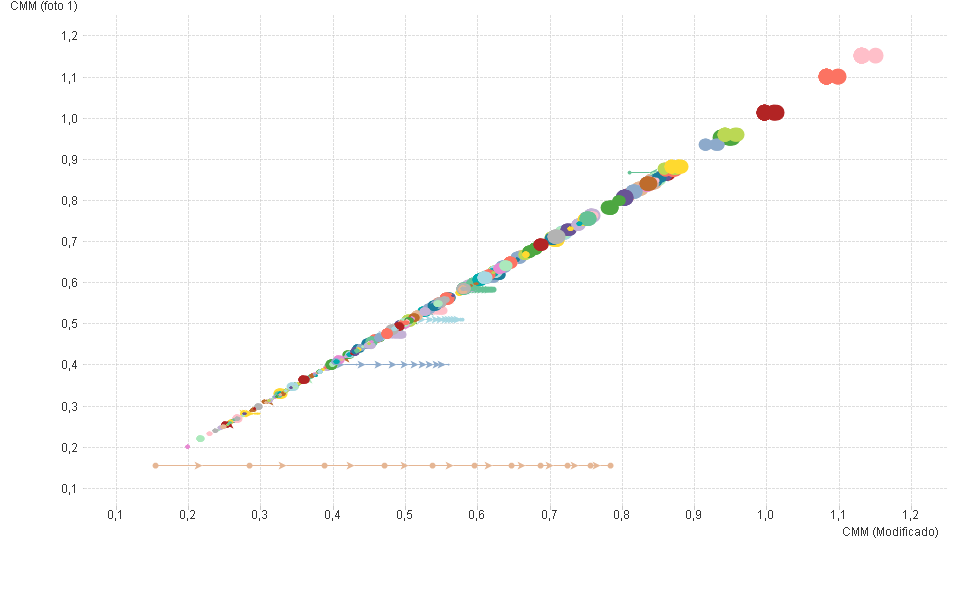
\includegraphics[width=1\textwidth]{IMG/comparativa cmm -cmm foto 10.png}
\caption{Zoom de las primeras posiciones}
\label{fig:Zoom de las primeras posiciones}
\end{figure}

\\



\subsection{Escalando Posiciones}

Una de las consignas del trabajo era encontrar una tecnica para hacer escalar en el ranking a un \textbf{equipo}, para lograr esto tenemos dos alternativas. \\


\subsubsection{El torneo ya finalizo}

En este escenario el torneo se encuentra finalizado y los resultados no pueden modificarse. Lo que proponemos es ver si modificando el orden de los partidos podemos influir en el ranking de un equipo. Para esto vamos a modificar el orden de sus victorias de forma tal de encontrar una que resulte en una mejoría de su ranking. \\


\subsubsection{Agregando partidos}

En este caso vamoa a analizar si podemos influir positivamente en el ranking a favor de un equipo, minimizando la cantidad de partidos ganados. \\

Nuestra teoría es que tomando el conjunto de equipos que perdio contra el seleccionado y haciendolos jugar y ganar a los principales del ranking, vamos a lograr que nuestro equipo mejore en la tabla de posiciones. \\



\subsection{Análisis Cuantitativo}


Vamos a estudiar la eficiencia de ambas tecnicas incrementando y variando los volúmenes de datos. La idea es repetir el cómputo de los rankings para la misma instancia de datos al azar, y posteriormente ir incrementando la cantidad de datos.

Nuestra hipótesis es el que método de basado en \textbf{WP} va a tardar lo mismo para instancias de datos iguales, y se irá incrementando de forma casi lineal a medida que incrementemos los datos. En cambio con \textbf{CMM} basando en \textbf{Eliminación Gaussiana} y \textbf{Cholesky} esperamos que difieran en para las mismas intancias. Nuestra hipótesis sobre esto es que la implementación de \textbf{Cholesky} va a demorar menos tiempo.


 




